\begin{figure}[t]
    \begin{minipage}[c]{0.48\textwidth}
    \begin{center}
        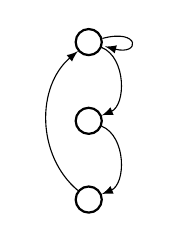
\begin{tikzpicture}[>=latex]
            \node[draw, thick, circle, radius=0.4] (a) at (0,0) {$\cX\cH\cH$};
            \node[draw, thick, circle, radius=0.4] (b) at (0,-1) {$\cH\cH\cM$};
            \node[draw, thick, circle, radius=0.4] (c) at (0,-2) {$\cH\cM\cH$};
            \draw[->] (a) edge [loop right] node[right] {$\cH$} (a);
            \draw[->] (a) edge [bend left=67.5] node[right] {$\cM$} (b);
            \draw[->] (b) edge [bend left=67.5] node[right] {$\cH$} (c);
            \draw[->] (c) edge [bend left=50] node[left] {$\cH$} (a);
        \end{tikzpicture}

        (Example~\ref{ex:auto-kill})\\[1pt]
        $\lambda^{\strat} = \overbar{\binom{1}{3}}^{\text{Kill}}$
    \end{center}
\end{minipage}
%
    \begin{minipage}[c]{0.48\textwidth}
    \begin{center}
        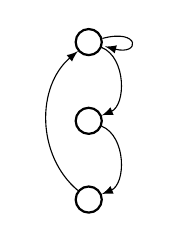
\begin{tikzpicture}[>=latex]
            \node[draw, thick, circle, radius=0.4] (a) at (0,0) {$\cX\cT\cH$};
            \node[draw, thick, circle, radius=0.4] (b) at (0,-1) {$\cT\cH\cM$};
            \node[draw, thick, circle, radius=0.4] (c) at (0,-2) {$\cH\cM\cR$};
            \draw[->] (a) edge [loop right] node[right] {$\cH$} (a);
            \draw[->] (a) edge [bend left=67.5] node[right] {$\cM$} (b);
            \draw[->] (b) edge [bend left=67.5] node[right] {$\cR$} (c);
            \draw[->] (c) edge [bend left=50] node[left] {$\cH$} (a);
        \end{tikzpicture}

        (Example~\ref{ex:auto-skip})\\[1pt]
        $\lambda^{\strat} = \overbar{\binom{1}{3}}^{\text{Skip-Next}}$
    \end{center}
\end{minipage}
%
    \caption{Automata $\GG{\lambda^{\strat}}$ for Examples 1 and 2.}
    \label{fig:min-graph}
\end{figure}
%
Any \ewhc{}, as presented in Definition~\ref{def:new-mk}, can be systematically represented using an \emph{automaton}.
In this paper we build upon the \tool{} automaton model presented in~{\cite{Vreman:2022}}.
Here, a (minimal) automaton $\GG{\lambda^\strat} = \left(\VV{\lambda^\strat}, \EE{\lambda^\strat}\right)$ associated to $\lambda^\strat$ consists of a set of vertices ($\VV{\lambda^\strat}$) and a set of directed labeled edges ($\EE{\lambda^\strat}$). 
Each vertex $v_i \in \VV{\lambda^\strat}$ corresponds to a sequence (word) of outcomes of the extended weakly-hard task executions. 
Trivially, there exists no vertices for words that do not satisfy the \ewhc{}.
A directed labeled edge $e_{i, j} = \left(v_i, v_j, \alpha \right) \in \EE{\lambda^\strat}$ (also denoted \emph{transition}) connects two vertices if and only if the outcome $\alpha \in \Sigma\left(\strat\right)$ -- the edge's label -- appended to the tail vertex's word representation ($v_i$) would result in the word equivalent to the one of the head vertex ($v_j$).
Thus, a random walk in the automaton corresponds to a random word satisfying the \ewhc{}.
In particular, all the walks in the automaton corresponds to \emph{all} words in $\sset{}{\lambda^{\strat}}$.

The \tool{} automaton model only operate on the binary alphabet $\Sigma = \left\{\cM, \cH\right\}$. 
To deal with the discrepancy between the \tool{} automaton model and the \ewhc{}, we introduce an additional auxiliary character $\cT$ to represent all outcomes where a job is completed (ergo; $\cT = \left\{ \cH,\, \cR \right\}$).
Thus, we first construct the automaton using the binary alphabet $\Sigma = \{\cM, \cT\}$ and then perform a post-processing step where Rule~\ref{rule:R} is enforced (for the \tS{} strategy) and the transitions are corrected, i.e., switching the labels on some edges from $\cT$ to $\cH$ or $\cR$ respectively. 

\begin{example}%
    \label{ex:auto-kill}%
    Given an \ewhc{}, $\lambda^{\strat} = \overbar{\binom{1}{3}}^{\tK{}}$, the automaton $\GG{\lambda^{\strat}}$ is shown in the left-hand side of Figure~\ref{fig:min-graph}.
    The vertex represented by the word $\cX\cH\cH$ is obtained by merging $\cH\cH\cH$ and $\cM\cH\cH$.
\end{example}

\begin{example}%
    \label{ex:auto-skip}%
    Given an \ewhc{}, $\lambda^{\strat} = \overbar{\binom{1}{3}}^{\tS{}}$, the automaton $\GG{\lambda^{\strat}}$ is shown in the right-hand side of Figure~\ref{fig:min-graph}.
\end{example}

The minimal automaton for \tK{} and \tS{} in Figure~\ref{fig:min-graph} have identical number of vertices but slightly different transitions.
This is not a coincidence, but follows directly from Definition~\ref{def:new-mk} and the extended alphabet $\Sigma\left(\strat\right)$.
Since we build the automaton using the job completion character $\cT$, both automata will always have the same structure.
It is only the first job completion, after a period of no job completions ($\cM$), that differ.
We emphasise that despite the extended automaton model appear similar for the \tK{} and \tS{} strategies, the differing transitions of the two automata significantly affect the corresponding closed-loop systems, as will be clear in Section~\ref{sec:stability}.

The \tool{} automaton model can also handle the case where a task $\tau$ is subject to a set of multiple constraints.
Intuitively, building upon Definition~\ref{def:satisfaction}, the satisfaction set of $\Lambda^{\strat}$ can be derived as follows:
%
\begin{equation}
    \label{eq:satisfaction-multi}
    \sset{N}{\Lambda^{\strat}} = \bigcap_{\lambda^{\strat}_i \in \Lambda^{\strat}_0} \sset{N}{\lambda^{\strat}_i}, \quad N \geq 1.
\end{equation}
%
With the notion of a satisfaction sets for sets of \ewhc{}, it is trivial to see that the domination relations also hold (Definition~\ref{def:domination}).
Since the stability analysis presented in this paper is invariant to the type (and amount) of constraints acting on the control task $\tau$, we henceforth say that $\tau$ is subject to a set of \ewhc{} $\Lambda^\strat$ (unless stated otherwise).


\subsection{Dynamic Model of an Automaton}
\label{ssec:dynamicgraph}
%
Extracting all the transitions in $\EE{\Lambda^\strat}$ corresponding to a character $\alpha \in \Sigma\left(\strat\right)$ yields what is generally known as a \emph{directed adjacency matrix}~\cite{xu2012matrix}, denoted here as a \emph{transition matrix}.
\begin{definition}[Transition matrix]%
    \label{def:transition}%
    Given an automaton $\GG{\Lambda^\strat}$, the \emph{transition matrix} $F_{\alpha} ( \GG{\Lambda^\strat} ) \in \R^{\abs{\VV{\Lambda^\strat}} \times \abs{\VV{\Lambda^\strat}}}$ for $\alpha\in\Sigma\left(\strat\right)$, is computed as $F_{\alpha} ( \GG{\Lambda^\strat} ) = \{f_{i,j}(\alpha)\}$ with
    %
    \begin{equation*}
        f_{i,j}\funof{\alpha}=
        \begin{cases}
            1, &\text{ if } \exists \, e=(v_j,v_i,\alpha) \in \EE{\Lambda^\strat} \\
            0, &\text{ otherwise.}
        \end{cases}
        \end{equation*}%
\end{definition}
%
Since there can exist \emph{at most one} successor from each vertex with a transition labeled with $\alpha$, the transition matrix $F_\alpha$ will have a column sum of either 1 or 0.
We introduce a vector $q_t\in \R^{n_{\VV{}}}$ called \emph{G-state}, with $n_{\VV{}} =\abs{\VV{\Lambda^\strat}}$, representing the state of the given automaton $\GG{\Lambda^\strat}$, which is associated to the interval $\pi_t$.
%
\begin{definition}[G-state]%
    \label{def:qt}%
    Given an automaton $\GG{\Lambda^\strat} = (\VV{\Lambda^\strat}, \EE{\Lambda^\strat})$ and a word $w = \langle \alpha_1,\alpha_2,\dots,\alpha_N \rangle \in \Sigma\left( \strat \right)^N$, for $k = \abs{v},\,\, v\in\VV{\Lambda^\strat}$, we define $q_t\in \R^{n_{\VV{}}}$, where the $i$-th element $q_{t,i}$ is defined as:
    \begin{equation*}
        q_{t,i}=
        \begin{cases}
            1, &\text{ if } \langle \alpha_{t-k},\dots,\alpha_{t-1} \rangle \equiv v_i \in \VV{\Lambda^\strat} \\
            0, &\text{otherwise}.
        \end{cases}
    \end{equation*}
\end{definition}
%
The G-state $q_t$ is the vector representation of the vertex \emph{left} at step $t$: here, $q_t=0$ means that the transition at step $t-1$ was infeasible for the automaton. 
Given an arbitrary string $w=\langle \alpha_1,\dots,\alpha_t,\dots \rangle$, the G-state dynamics is defined as $q_{t+1} = F_{\alpha_t}\funof{\GG{\Lambda^\strat}} \cdot q_t$, and the following property holds~\cite{xu2012matrix}.
%
\begin{lemma}[Infeasible sequence]%
    \label{cor:Fseqnotinlambda}%
    If $\langle \alpha_1,\dots,\alpha_t,\dots \rangle \notin \sset{N}{ \Lambda^\strat }$, then 
    \begin{equation*}
        F_{\alpha_N}\funof{\GG{\Lambda^\strat}} \cdots F_{\alpha_2}\funof{\GG{\Lambda^\strat}} \cdot F_{\alpha_1}\funof{\GG{\Lambda^\strat}} = 0.
    \end{equation*}
\end{lemma}
Thus, if $q_t=0$ for any $t$, then $q_{t'}=0$ for $t' \geq t$.
